% This is LLNCS.DEM the demonstration file of
% the LaTeX macro package from Springer-Verlag
% for Lecture Notes in Computer Science,
% version 2.4 for LaTeX2e as of 16. April 2010
%
\documentclass{llncs}
%
\usepackage{makeidx}  % allows for indexgeneration
\usepackage{amsmath}
\usepackage{amssymb}
\usepackage{graphicx}
%
\begin{document}
%
\mainmatter              % start of the contributions
%
\title{Case Study of Liveness Verification in IronFleet}
%
\author{Lucas Pe\~{n}a and Manasvi Saxena}
%
\institute{University of Illinois at Urbana-Champaign, \\
\email{\{lpena7, msaxena2\}@illinios.edu}}

\maketitle              % typeset the title of the contribution

\begin{abstract}
  As more complicated software systems are becoming prevalent in today's world,
  more sophisticated program verification techniques are needed to reason about
  these. In particular, verification of liveness properties, or asserting that a
  property must occur, is traditionally difficult. In this paper, we survey the
  IronFleet methodology~\cite{ironfleet}, a technique for building distributed
  systems that are provably correct, as it applies to verification of liveness
  properties. We consider the embedding of the Temporal Logic of Actions used in
  IronFleet, and discuss some limitations in their implementation.
\end{abstract}
%
\section{Introduction}
Many tools are used for ensuring correctness of a system. These range from
testing to full formal verification. Formal verification is obviously the most
desirable, but the most difficult in practice. One generally requires a formal
specification of the property he or she is proving correct. This often makes
large-scale formal verification a difficult and cumbersome task. Still, many
success stories exist in the area of large-scale formal verification, such as
the CompCert compiler~\cite{compcert} and the Verve operating
system~\cite{verve}. However, formal verification of large-scale distributed
systems are basically nonexistent, due to the difficulty in verifying liveness
properties rather than safety properties.

\subsection{Safety Verification}
Most formal verification techniques focus on verifying safety
properties. Informally, a safety property asserts that ``nothing bad ever
happens.'' More formally, this means if a system violates a safety property $P$
at any point in its execution, the full execution must also violate $P$. Thus,
safety properties have \textit{finite length counterexamples}. Because of this
crucial fact, many techniques such as model checking and monitoring focus
specifically on verifying safety properties.

\subsection{Liveness Verification}
In contrast, a liveness property asserts that ``somerthing good will happen.''
This means one must have the entire execution in hand in order to assert the
absence of a liveness property. Thus, liveness properties have \textit{infinite
  length counterexamples}.  Thus, though liveness verification has the same
theoretical complexity as safety verification~\cite{simulation-liveness}, in
practice it is much more difficult to verify liveness properties. Clearly, it is
fruitless to do any kind of brute force search for the absence of such a
counterexample. Instead, specific techniques for verifying liveness properties
have been developed, which we discuss in Section~\ref{sec:rel-work}.

The IronFleet methodology uses a proof strategy based on Lamport's Temporal
Logic of Actions (TLA) that chains smaller proofs together to assert the
existence of some final condition (see
Section~\ref{sec:liveness-ironfleet}). Unlike the related work on liveness
verification, IronFleet is the first to verify nontrivial liveness properties on
a large-scale distributed system.
%
\section{IronFleet}
Microsoft's Ironfleet methodology, is claimed to be the first complete suite of 
solutions that can perform automated, machine checked verification 
in non trivial, and distributed systems. Ironfleet supports 
verification of both safety and liveness properties. We discuss, in detail, the 
approach used by Ironfleet. We use the IronRSL system for further analysis.

\subsection{Dafny}
Dafny is a programming language with built-in specification constructs. The Dafny
ecosystem consists of a static program verifier used for proving correctness of
programs and their specifications. The ironfleet methodology relies 
on Dafny for describing specifications and proving correctness of implementations. 

\subsection{End-to-end Verification}
Verification techniques employed in the Ironfleet suite are not novel. Ironfleet's 
motivation is to use existing verification techniques on large, complicated, and practical distributed
systems. In this regard, Ironfleet breaks new ground. The software codebase that Ironfleet
has been used to verify have features and performance comparable to similar, non-verified solutions. 
Ironfleet supports both safety and liveness verification. When liveness verification is taken into account, 
the Ironfleet methodology is supposedly the first succesful attempt at verifying liveness of both
the protocol, and the conforming implementation. 

Ironfleet achieves end to end verification of distributed systems by structing the system into layers, and 
developing proofs on them. Ironfleet blends TLA-style refinement to reason about protocol-level concurrency, 
while ignoring the implementation. It then uses Floyd-Hoare style verification to reason about implementation,
while ignoring concurrency. This allows the Ironfleet to reason about both the high-level specification, and
the impementation. We briefly descirbe the layers used in Ironfleet to structure reasoning about systems - 
\begin{\itemize}
\item At the top layer, a high level specification for the entire system's behavior is provided. 
\item The middle layer contains the specification for the distributed protocol implemented by the
    system. Ironfleet TLA-style techniques uses TLA style techniques to prove that the middle layer 
    refines the top layer.
\item The third layer contains the implementation details of the protocol, or the code to be run on each node.
    Ironfleet uses refinement to prove that the implementation layer refines the protocol description layer. 
\end{\itemize}

The layering methodology allows Ironfleet to deal with complexities of the system effectively. 


\subsection{Refinement}
\subsection{Liveness Verification in IronFleet}\label{sec:liveness-ironfleet}
\subsubsection{Limitations}
%
\section{Temporal Logic of Actions}
The Temporal Logic of Actions (TLA)~\cite{tla-lamport} is an extension of Linear Temporal
Logic introduced to reason about concurrent systems. TLA introduces ``primed''
variables, which represents the value of a variable in the next state. For
example, the TLA \textit{action} $$x' = x + y$$ specifies that the value of $x$
in the next state is equal to the value of $x + y$ in the current state. An
action is satisfied by a pair of states $\langle s, t \rangle$, where $s$ is a
valuation on the unprimed variables and $t$ is a valuation on the primed
variables. The notion of primed variables allow us to specify a rich class of
formulas not expressible in normal LTL.

First, we can represent the action $Unchanged\;f \equiv f' = f$ for any 
function $f$  without primed variables, which states that $f$ is a
stuttering step. Using this, we can also represent the derived actions
$[\mathcal A]_f$ and $\langle \mathcal A \rangle_f$ for any action
$\mathcal A$. These respectively represent that an action either satisfies $\mathcal A$ or
stutters (w.r.t. $f$), and that an action that satisfies $\mathcal A$
necessarily changes $f$. These are defined as follows:
\begin{align*}
  [\mathcal A]_f \equiv \mathcal A \vee Unchanged\;f \hspace{1.5cm}
  & \langle \mathcal A \rangle_f \equiv \mathcal A \wedge \neg(Unchanged\;f)
\end{align*}
TLA also introduces the action $Enabled\;\mathcal A$ which specifies that for
any $s$, there is a $t$ such that $\langle s, t \rangle$ satisfies $\mathcal A$.

TLA \textit{formulas} add the temporal operator $\square$, like in LTL. In
addition, quantification over formulas is allowed. Derived formulas such as
$\lozenge$ are as in LTL. Other derived formulas include $F \leadsto G$
(\textit{leads to}), WF$_f(\mathcal A)$ (\textit{weak fairness}), and
SF$_f(\mathcal A)$ (\textit{strong fairness}). These are defined as follows:
\begin{align*}
  F \leadsto G &\equiv \square(F \Rightarrow \lozenge G) \\
  \text{WF}_f(\mathcal A) &\equiv \square\lozenge\langle\mathcal A\rangle_f \vee \square\lozenge\neg Enabled\;\langle\mathcal A\rangle_f \\
  \text{SF}_f(\mathcal A) &\equiv \square\lozenge\langle\mathcal A\rangle_f \vee \lozenge\square\neg Enabled\;\langle\mathcal A\rangle_f
\end{align*}
For use in verification, these derived formulas can express most liveness
properties a user may want to express. Of course, for verification, we need
proof rules allowing us to reason about these formulas, which we present below.

\begin{figure}
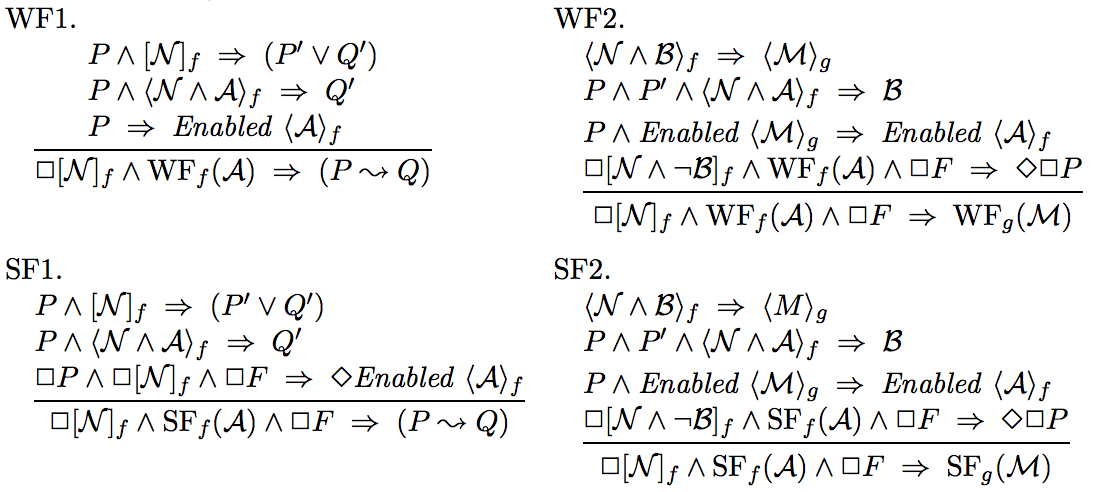
\includegraphics[scale=0.6]{tla-rules}
\centering
\end{figure}

These rules allow us to reason about both strong fairness and weak fairness,
both as a hypothesis and a conclusion. The use of these rules is demonstrated
via a simple program that nondeterministically chooses one of two variables to
increment ad infinitum. One can define a naive implementation of this program,
as well as a more complex one using semaphores.

The TLA rules above can be used to prove weak fairness of the first
implementation, strong fairness of the second, and it can even be used to prove
that the semaphore implementation is a refinement of the naive implementation.
Notably, all four of the above rules must be used for these proofs.


\section{Related Work}\label{sec:rel-work}
Though verification of liveness properties is notoriously difficult and rare,
the IronFleet methodology was of course not the first to formally verify
liveness properties. Previous techniques include BDD-based model
checking~\cite{Ravi2000} as well as converting liveness properties to safety
properties~\cite{Schuppan2006}.

BDD-based model checking relies on Binary Decision Diagrams (BDDs) as a data
structure that can be used to represent boolean functions. Unfortunately, the
size of the BDD can scale exponentially with the size of the system, so this
approach is not scalable.

Converting a liveness property to a safety property is an attractive idea, since
it opens up the use of existing algorithms to verify safety properties. However,
the translation used in~\cite{Schuppan2006} incurs a large increase in problem
size, making this technique not scalable as well.

\section{Conclusion}

%
% ---- Bibliography ----
%
\bibliographystyle{ieeetr}

\bibliography{references}

\end{document}
